% !TeX program = xelatex
%
% МЛГ-версия лекции «Введение в машинное обучение».
% Направление «Цифровая лингвистика и локализация», магистратура лингвистики.
%
% Сборка:  xelatex mlg_intro_ml.tex   (дважды, ради оглавления)
% Графика: fig/*.pdf, строится скриптом собрать_иллюстрации.py на реальном
%          учебном корпусе курса. Придуманных чисел на слайдах нет.
%
\documentclass[aspectratio=169,12pt]{beamer}

% Общая преамбула лекций курса. Подключается после \documentclass:
%
%     \documentclass[aspectratio=169,12pt]{beamer}
%     % Общая преамбула лекций курса. Подключается после \documentclass:
%
%     \documentclass[aspectratio=169,12pt]{beamer}
%     % Общая преамбула лекций курса. Подключается после \documentclass:
%
%     \documentclass[aspectratio=169,12pt]{beamer}
%     \input{mlg_preamble}
%
% Здесь только оформление и макросы — ни \title, ни текста слайдов, чтобы
% пять презентаций курса выглядели одинаково и правились в одном месте.
%
\usepackage{fontspec}
\usepackage{polyglossia}
\setmainlanguage{russian}
\setotherlanguage{english}
\setmainfont{Calibri}
\setsansfont{Calibri}
\setmonofont{Consolas}[Scale=0.92]

\usepackage{graphicx}
\usepackage{booktabs}
\usepackage{array}

% ---------------------------------------------------------------- оформление
\definecolor{ink}{HTML}{1B2433}
\definecolor{navy}{HTML}{2B4C6F}
\definecolor{brick}{HTML}{B03A2B}
\definecolor{moss}{HTML}{3E7D5A}
\definecolor{plum}{HTML}{6B5B95}
\definecolor{ash}{HTML}{8B9299}
\definecolor{paper}{HTML}{ECEFF3}

\usetheme{default}
\usecolortheme{default}
\setbeamercolor{structure}{fg=navy}
\setbeamercolor{frametitle}{fg=navy}
\setbeamercolor{normal text}{fg=ink}
\setbeamercolor{itemize item}{fg=navy}
\setbeamercolor{itemize subitem}{fg=ash}
\setbeamerfont{frametitle}{size=\Large,series=\bfseries}
\setbeamerfont{framesubtitle}{size=\small,series=\mdseries}
\setbeamercolor{framesubtitle}{fg=ash}
\setbeamertemplate{navigation symbols}{}
\setbeamertemplate{itemize item}{\raisebox{0.15ex}{\tiny$\bullet$}}
\setbeamertemplate{itemize subitem}{\raisebox{0.15ex}{\tiny--}}
\setbeamersize{text margin left=1.1cm, text margin right=1.1cm}

\setbeamertemplate{footline}{%
  \hbox{\begin{beamercolorbox}[wd=\paperwidth,ht=2.6ex,dp=1.4ex,leftskip=1.1cm,%
        rightskip=1.1cm]{}%
    {\color{ash}\scriptsize Основы машинного обучения \quad·\quad
     Цифровая лингвистика и локализация}\hfill
    {\color{ash}\scriptsize\insertframenumber}%
  \end{beamercolorbox}}}

% Врезка: связь слайда с лабораторной или с работой переводчика.
% Ширина считается точно: colorbox добавляет \fboxsep с каждой стороны,
% поэтому parbox должен быть на 2\fboxsep уже текстового поля — иначе
% на каждом слайде вылезает overfull hbox.
\newcommand{\врезка}[1]{%
  \par\vspace{0.5ex}\noindent
  \colorbox{paper}{%
    \parbox{\dimexpr\textwidth-2\fboxsep\relax}{%
      \vspace{0.7ex}\small #1\vspace{0.7ex}}}\par}

% Колонка таблицы заданной доли ширины, без растягивания пробелов.
% Объявлять её нужно здесь: внутри frame beamer пересканирует тело кадра,
% и #1 в определении вызывает «Illegal parameter number».
\newcolumntype{Л}[1]{>{\raggedright\arraybackslash}p{#1\textwidth}}

% Ссылка на интерактивную страницу к слайду. Playground'ы считают те же
% числа на том же корпусе, что и лабораторные, поэтому на них можно
% ссылаться прямо с лекции, не оговаривая расхождений.
\hypersetup{colorlinks=true,urlcolor=moss,linkcolor=moss}
\newcommand{\playground}[3]{%
  \par\vspace{0.4ex}%
  {\footnotesize\color{ash}$\rightarrow$~\href{#1}{\bfseries #2} — #3\par}}

\newcommand{\кейс}[1]{{\color{brick}\small\textbf{#1}}}
\newcommand{\числ}[1]{{\color{navy}\bfseries #1}}

%
% Здесь только оформление и макросы — ни \title, ни текста слайдов, чтобы
% пять презентаций курса выглядели одинаково и правились в одном месте.
%
\usepackage{fontspec}
\usepackage{polyglossia}
\setmainlanguage{russian}
\setotherlanguage{english}
\setmainfont{Calibri}
\setsansfont{Calibri}
\setmonofont{Consolas}[Scale=0.92]

\usepackage{graphicx}
\usepackage{booktabs}
\usepackage{array}

% ---------------------------------------------------------------- оформление
\definecolor{ink}{HTML}{1B2433}
\definecolor{navy}{HTML}{2B4C6F}
\definecolor{brick}{HTML}{B03A2B}
\definecolor{moss}{HTML}{3E7D5A}
\definecolor{plum}{HTML}{6B5B95}
\definecolor{ash}{HTML}{8B9299}
\definecolor{paper}{HTML}{ECEFF3}

\usetheme{default}
\usecolortheme{default}
\setbeamercolor{structure}{fg=navy}
\setbeamercolor{frametitle}{fg=navy}
\setbeamercolor{normal text}{fg=ink}
\setbeamercolor{itemize item}{fg=navy}
\setbeamercolor{itemize subitem}{fg=ash}
\setbeamerfont{frametitle}{size=\Large,series=\bfseries}
\setbeamerfont{framesubtitle}{size=\small,series=\mdseries}
\setbeamercolor{framesubtitle}{fg=ash}
\setbeamertemplate{navigation symbols}{}
\setbeamertemplate{itemize item}{\raisebox{0.15ex}{\tiny$\bullet$}}
\setbeamertemplate{itemize subitem}{\raisebox{0.15ex}{\tiny--}}
\setbeamersize{text margin left=1.1cm, text margin right=1.1cm}

\setbeamertemplate{footline}{%
  \hbox{\begin{beamercolorbox}[wd=\paperwidth,ht=2.6ex,dp=1.4ex,leftskip=1.1cm,%
        rightskip=1.1cm]{}%
    {\color{ash}\scriptsize Основы машинного обучения \quad·\quad
     Цифровая лингвистика и локализация}\hfill
    {\color{ash}\scriptsize\insertframenumber}%
  \end{beamercolorbox}}}

% Врезка: связь слайда с лабораторной или с работой переводчика.
% Ширина считается точно: colorbox добавляет \fboxsep с каждой стороны,
% поэтому parbox должен быть на 2\fboxsep уже текстового поля — иначе
% на каждом слайде вылезает overfull hbox.
\newcommand{\врезка}[1]{%
  \par\vspace{0.5ex}\noindent
  \colorbox{paper}{%
    \parbox{\dimexpr\textwidth-2\fboxsep\relax}{%
      \vspace{0.7ex}\small #1\vspace{0.7ex}}}\par}

% Колонка таблицы заданной доли ширины, без растягивания пробелов.
% Объявлять её нужно здесь: внутри frame beamer пересканирует тело кадра,
% и #1 в определении вызывает «Illegal parameter number».
\newcolumntype{Л}[1]{>{\raggedright\arraybackslash}p{#1\textwidth}}

% Ссылка на интерактивную страницу к слайду. Playground'ы считают те же
% числа на том же корпусе, что и лабораторные, поэтому на них можно
% ссылаться прямо с лекции, не оговаривая расхождений.
\hypersetup{colorlinks=true,urlcolor=moss,linkcolor=moss}
\newcommand{\playground}[3]{%
  \par\vspace{0.4ex}%
  {\footnotesize\color{ash}$\rightarrow$~\href{#1}{\bfseries #2} — #3\par}}

\newcommand{\кейс}[1]{{\color{brick}\small\textbf{#1}}}
\newcommand{\числ}[1]{{\color{navy}\bfseries #1}}

%
% Здесь только оформление и макросы — ни \title, ни текста слайдов, чтобы
% пять презентаций курса выглядели одинаково и правились в одном месте.
%
\usepackage{fontspec}
\usepackage{polyglossia}
\setmainlanguage{russian}
\setotherlanguage{english}
\setmainfont{Calibri}
\setsansfont{Calibri}
\setmonofont{Consolas}[Scale=0.92]

\usepackage{graphicx}
\usepackage{booktabs}
\usepackage{array}

% ---------------------------------------------------------------- оформление
\definecolor{ink}{HTML}{1B2433}
\definecolor{navy}{HTML}{2B4C6F}
\definecolor{brick}{HTML}{B03A2B}
\definecolor{moss}{HTML}{3E7D5A}
\definecolor{plum}{HTML}{6B5B95}
\definecolor{ash}{HTML}{8B9299}
\definecolor{paper}{HTML}{ECEFF3}

\usetheme{default}
\usecolortheme{default}
\setbeamercolor{structure}{fg=navy}
\setbeamercolor{frametitle}{fg=navy}
\setbeamercolor{normal text}{fg=ink}
\setbeamercolor{itemize item}{fg=navy}
\setbeamercolor{itemize subitem}{fg=ash}
\setbeamerfont{frametitle}{size=\Large,series=\bfseries}
\setbeamerfont{framesubtitle}{size=\small,series=\mdseries}
\setbeamercolor{framesubtitle}{fg=ash}
\setbeamertemplate{navigation symbols}{}
\setbeamertemplate{itemize item}{\raisebox{0.15ex}{\tiny$\bullet$}}
\setbeamertemplate{itemize subitem}{\raisebox{0.15ex}{\tiny--}}
\setbeamersize{text margin left=1.1cm, text margin right=1.1cm}

\setbeamertemplate{footline}{%
  \hbox{\begin{beamercolorbox}[wd=\paperwidth,ht=2.6ex,dp=1.4ex,leftskip=1.1cm,%
        rightskip=1.1cm]{}%
    {\color{ash}\scriptsize Основы машинного обучения \quad·\quad
     Цифровая лингвистика и локализация}\hfill
    {\color{ash}\scriptsize\insertframenumber}%
  \end{beamercolorbox}}}

% Врезка: связь слайда с лабораторной или с работой переводчика.
% Ширина считается точно: colorbox добавляет \fboxsep с каждой стороны,
% поэтому parbox должен быть на 2\fboxsep уже текстового поля — иначе
% на каждом слайде вылезает overfull hbox.
\newcommand{\врезка}[1]{%
  \par\vspace{0.5ex}\noindent
  \colorbox{paper}{%
    \parbox{\dimexpr\textwidth-2\fboxsep\relax}{%
      \vspace{0.7ex}\small #1\vspace{0.7ex}}}\par}

% Колонка таблицы заданной доли ширины, без растягивания пробелов.
% Объявлять её нужно здесь: внутри frame beamer пересканирует тело кадра,
% и #1 в определении вызывает «Illegal parameter number».
\newcolumntype{Л}[1]{>{\raggedright\arraybackslash}p{#1\textwidth}}

% Ссылка на интерактивную страницу к слайду. Playground'ы считают те же
% числа на том же корпусе, что и лабораторные, поэтому на них можно
% ссылаться прямо с лекции, не оговаривая расхождений.
\hypersetup{colorlinks=true,urlcolor=moss,linkcolor=moss}
\newcommand{\playground}[3]{%
  \par\vspace{0.4ex}%
  {\footnotesize\color{ash}$\rightarrow$~\href{#1}{\bfseries #2} — #3\par}}

\newcommand{\кейс}[1]{{\color{brick}\small\textbf{#1}}}
\newcommand{\числ}[1]{{\color{navy}\bfseries #1}}


\title{Введение в машинное обучение}
\subtitle{Основные задачи и технологии интеллектуальной обработки данных}
\date{}
\author{}

\begin{document}

% =====================================================================
\begin{frame}[plain]
  \vspace{1.2cm}
  {\color{brick}\small\bfseries ОСНОВЫ МАШИННОГО ОБУЧЕНИЯ}

  \vspace{0.7cm}
  {\color{navy}\fontsize{30}{34}\selectfont\bfseries Введение в машинное обучение\par}

  \vspace{0.5cm}
  {\color{ink}\large Основные задачи и технологии интеллектуальной обработки данных\par}

  \vspace{1.0cm}
  {\color{ash} Версия для направления «Цифровая лингвистика и локализация».\\
   Все примеры и все числа на слайдах посчитаны на учебном корпусе курса:
   160 сегментов локализации, четыре типа контента.\par}
\end{frame}

% =====================================================================
\begin{frame}{Где эта лекция в курсе}
  Материал собран из трёх презентаций, и они не повторяют друг друга.

  \vspace{0.5em}
  \begin{columns}[T,onlytextwidth]
    \column{0.32\textwidth}
      {\color{navy}\bfseries 1. Введение в МО}\\[0.3em]
      {\small Эта лекция. Общая карта: какие бывают задачи и чем они
      отличаются друг от друга.}
    \column{0.32\textwidth}
      {\color{navy}\bfseries 2. Интеллектуальный анализ текстовых данных}\\[0.3em]
      {\small Работа с корпусом: сбор, форматы, выбросы, устройство нейрона,
      GPT и трансформер.}
    \column{0.32\textwidth}
      {\color{navy}\bfseries 3. Текст как данные}\\[0.3em]
      {\small То, на что опираются лабораторные: векторизация, метрики
      качества текста, разметка.}
  \end{columns}

  \vspace{1.2em}
  \врезка{\textbf{Зачем это знать лингвисту.} Вы не будете обучать модели.
  Вы будете решать, годится ли результат модели для проекта, и объяснять
  заказчику, почему он стоит столько, сколько стоит. Для этого нужно
  понимать, что модель в принципе умеет, а чего не умеет никогда.}
\end{frame}

% =====================================================================
\begin{frame}{Машинное обучение}
  \framesubtitle{англ. machine learning, ML}

  Класс методов искусственного интеллекта, характерная черта которых —
  \textbf{не прямое решение задачи, а обучение на примерах}.

  \vspace{0.6em}
  \begin{columns}[T,onlytextwidth]
    \column{0.47\textwidth}
      {\color{ash}\bfseries Программа по правилам}\\[0.4em]
      {\small Лингвист пишет: «кончается вопросительным знаком и короче
      пяти слов — значит интерфейс». Правила видны и правятся, но каждое
      написано руками.}
    \column{0.47\textwidth}
      {\color{navy}\bfseries Машинное обучение}\\[0.4em]
      {\small Лингвист размечает 160 сегментов по типам. Правила машина
      выводит сама. Написать их она не может — только применить.}
  \end{columns}

  \vspace{0.9em}
  \врезка{Оба подхода в курсе встретятся, и мы их сравним численно:
  в Л.р.\,№\,3 формальные проверки написаны по правилам, а модель
  перевода обучена на примерах.}
\end{frame}

% =====================================================================
\begin{frame}{Что нужно, чтобы машинное обучение состоялось}
  \begin{columns}[T,onlytextwidth]
    \column{0.30\textwidth}
      {\color{navy}\bfseries Данные}\\[0.4em]
      {\small Размеченные примеры. В нашем корпусе — 160 сегментов,
      у каждого проставлен тип контента.}\\[0.5em]
      {\color{brick}\small Это делает лингвист, и это самая дорогая часть.}
    \column{0.30\textwidth}
      {\color{navy}\bfseries Признаки}\\[0.4em]
      {\small Числа, которыми описан текст. Слова, буквосочетания, длина,
      наличие плейсхолдера.}\\[0.5em]
      {\color{brick}\small Здесь решается почти всё — увидим в Л.р.\,№\,1.}
    \column{0.30\textwidth}
      {\color{navy}\bfseries Алгоритм}\\[0.4em]
      {\small Способ связать признаки с ответом. Наивный Байес, дерево
      решений, логистическая регрессия.}\\[0.5em]
      {\color{ash}\small Меняется одной строкой кода.}
  \end{columns}

  \vspace{1.3em}
  \врезка{\textbf{Заранее о главном выводе первой лабораторной.}
  Смена алгоритма на том же корпусе дала прирост точности
  \числ{0{,}01}. Смена признаков — \числ{0{,}21}. Порядок величин
  разный, и это определяет, на что тратить время в проекте.}
\end{frame}

% =====================================================================
\begin{frame}{Машинное обучение и искусственный интеллект}
  \textbf{Искусственный интеллект} — широкая область: всё, что заставляет
  машину вести себя разумно, включая системы правил, планировщики,
  экспертные системы.

  \vspace{0.6em}
  \textbf{Машинное обучение} — её часть: методы, которые извлекают
  закономерность из данных.

  \vspace{0.6em}
  \textbf{Глубокое обучение} — часть машинного обучения: многослойные
  нейронные сети.

  \vspace{1.2em}
  \врезка{\textbf{Почему это важно проговорить.} Системы автоматического
  перевода прошли все три стадии: правила (до 1990-х), статистика
  (1990–2015), нейросети (с 2015). В отрасли до сих пор работают
  инструменты всех трёх поколений, и вы будете иметь дело с каждым.}
\end{frame}

% =====================================================================
\begin{frame}{Четыре направления машинного обучения}
  \begin{center}
    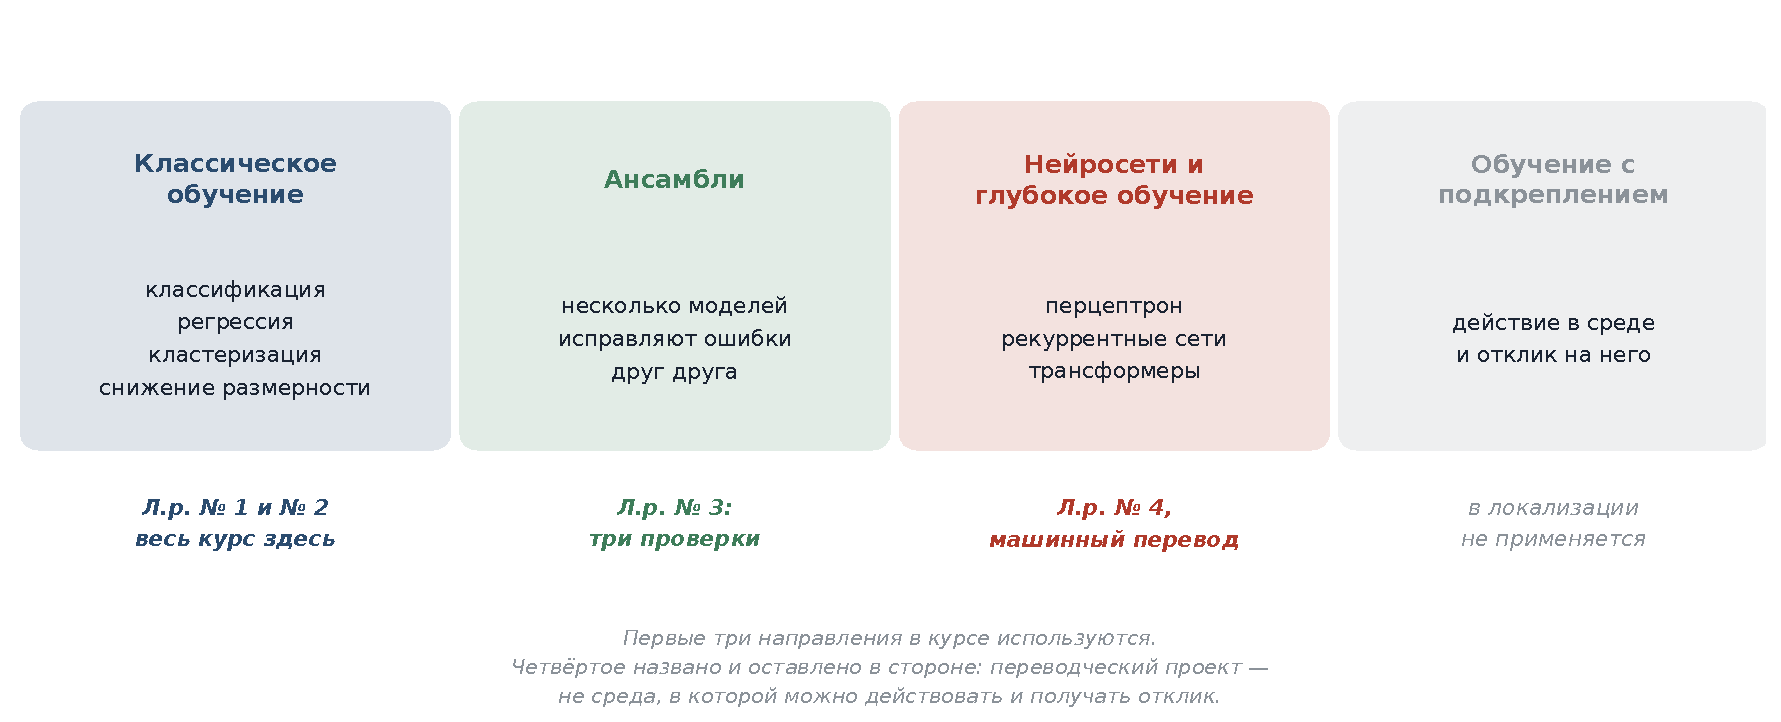
\includegraphics[width=0.96\textwidth]{fig/directions.pdf}
  \end{center}
\end{frame}

% =====================================================================
\begin{frame}{Классификация}
  \framesubtitle{обучение с учителем}

  Задача: отнести объект к одному из заранее известных классов.
  Классы задаёт человек, машина учится их различать по размеченным примерам.

  \vspace{0.9em}
  \кейс{Наша задача в Л.р.\,№\,1:} по тексту сегмента определить тип
  контента — \textbf{интерфейс}, \textbf{документация}, \textbf{маркетинг}
  или \textbf{юридический текст}.

  \vspace{0.9em}
  \врезка{\textbf{Зачем это нужно в проекте.} Перед началом работы
  приходит выгрузка на десятки тысяч строк без разделения. От типа
  контента зависит всё: кто переводит, по какому глоссарию, с каким
  тоном, какая ставка. Разбирать руками — это дни работы.}

  \vspace{0.8em}
  {\color{ash}\small Классы у нас равные — по 40 сегментов. Решение,
  всегда отвечающее самым частым классом, даёт \числ{0{,}25}.
  Всё, что ниже этого, бесполезно, какой бы сложности ни была модель.}
\end{frame}

% =====================================================================
\begin{frame}{Наивный Байес: с чего начинались спам-фильтры}
  Машина считает, \textbf{сколько раз слово встретилось} в письме, и по
  этим счётчикам оценивает вероятность того, что письмо — спам.

  \vspace{0.3em}
  \begin{center}
    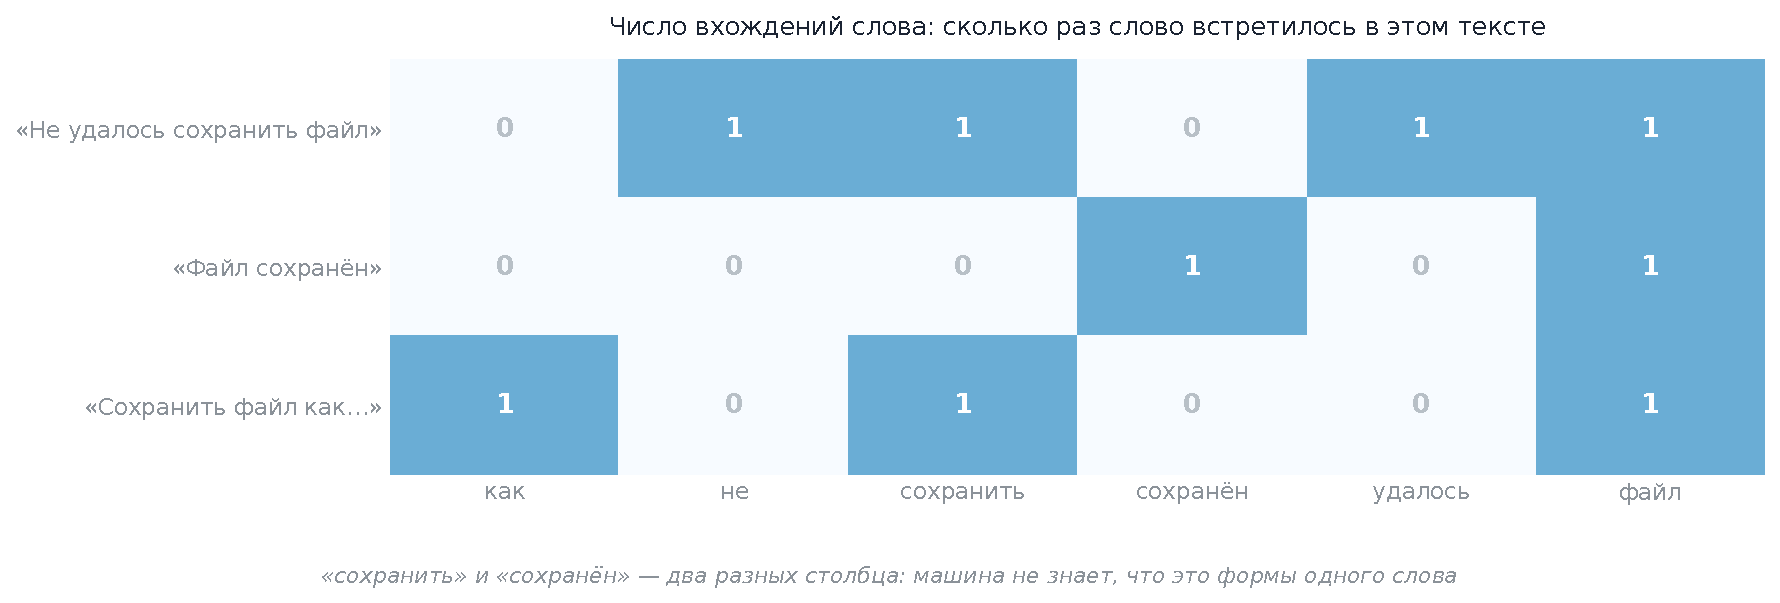
\includegraphics[width=0.76\textwidth]{fig/bagofwords.pdf}
  \end{center}

  \vspace{-0.5em}
  \врезка{Это представление называется \textbf{мешком слов}. Порядок слов
  теряется полностью: «не удалось подключиться» и «удалось не подключиться»
  дают одинаковый вектор. Для типа контента терпимо, для оценки перевода —
  уже нет, и в Л.р.\,№\,3 это станет принципиальным.}
\end{frame}

% =====================================================================
\begin{frame}{Тот же алгоритм на нашем корпусе}
  \begin{columns}[T,onlytextwidth]
    \column{0.46\textwidth}
      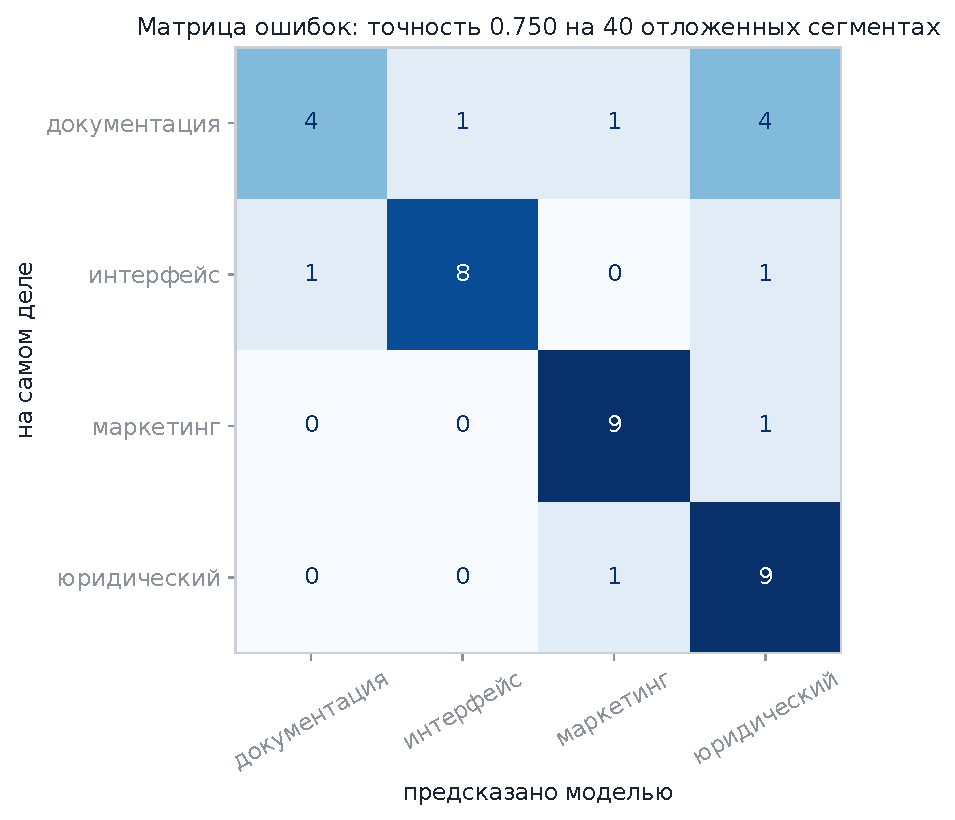
\includegraphics[width=\textwidth]{fig/confusion.pdf}
    \column{0.50\textwidth}
      \vspace{0.1cm}
      {\small
      \textbf{Матрица ошибок} показывает не только сколько ошибок, но и
      \emph{какие}: какой класс с каким смешивается.\par
      \vspace{0.7em}
      Диагональ — верные ответы. Всё вне её — то, что в проекте придётся
      переделывать руками.\par
      \vspace{0.7em}
      {\color{brick}\bfseries Читается по-лингвистически:} путаются
      документация, маркетинг и юридический текст — все трое состоят из
      полных предложений. Интерфейс не путается почти ни с чем: короткие
      безглагольные строки ни на что не похожи.}
  \end{columns}

  \playground{https://konkin-nikita.ru/gd_learn/vec/}{векторизация текста}%
  {та же матрица, но признаки переключаются на ходу.}
\end{frame}

% =====================================================================
\begin{frame}{Дерево решений: правила, которые можно прочесть}
  \begin{center}
    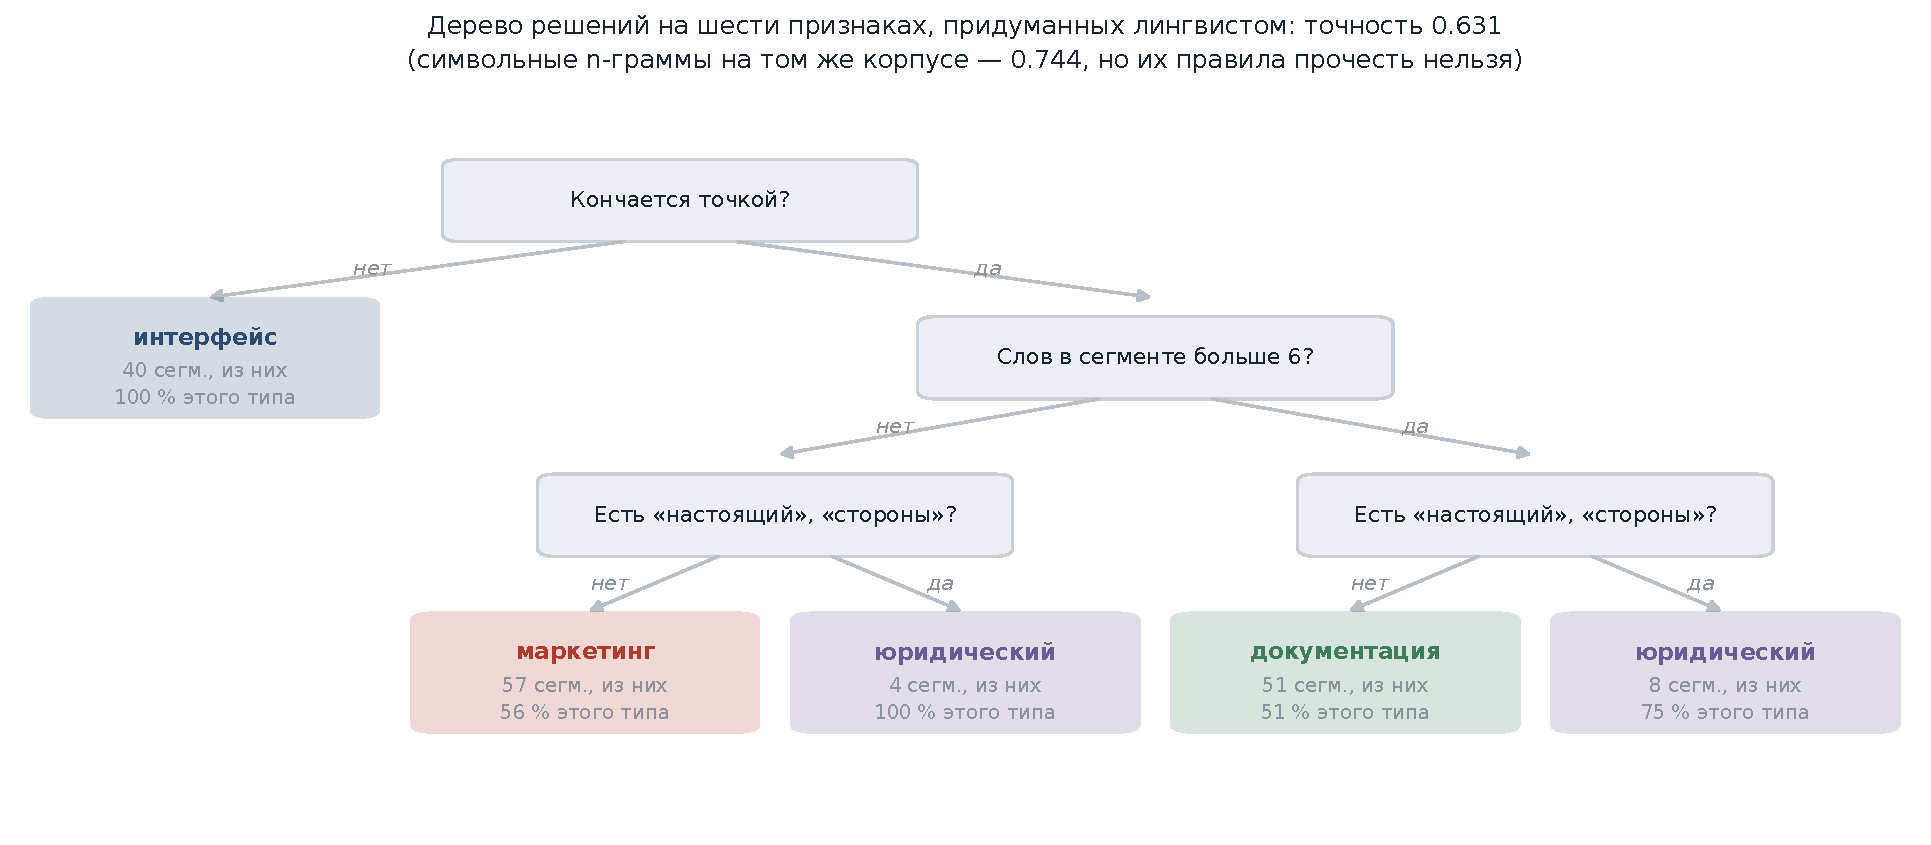
\includegraphics[width=0.93\textwidth]{fig/tree.pdf}
  \end{center}

  \vspace{-0.6em}
  {\small Шесть признаков придуманы лингвистом: длина, финальная точка,
  начальный инфинитив, плейсхолдер, обращение «вы», юридические маркеры.}
\end{frame}

% =====================================================================
\begin{frame}{Что мы узнали из дерева}
  \begin{columns}[T,onlytextwidth]
    \column{0.47\textwidth}
      {\color{moss}\bfseries Хорошая новость}\\[0.5em]
      {\small Машина сама вывела правила, под которыми подписался бы
      редактор: интерфейс не кончается точкой; юридический текст выдают
      «настоящий» и «стороны»; документация длиннее маркетинга.\par
      \vspace{0.6em}
      Такую модель можно показать заказчику и защитить.}
    \column{0.47\textwidth}
      {\color{brick}\bfseries Плохая новость}\\[0.5em]
      {\small Точность \числ{0{,}631}. Непрозрачная модель на символьных
      n-граммах даёт \числ{0{,}744} — и объяснить её решения нельзя.\par
      \vspace{0.6em}
      Выбор между понятностью и точностью — не техническая мелочь, а
      условие договора: за понятную модель платят, когда решение нужно
      обосновывать.}
  \end{columns}

  \vspace{0.35em}
  \врезка{В общей версии курса здесь пример про оценку кредитоспособности
  заёмщика. Механика та же и вывод тот же: вопросы дерева бывают адекватны
  человеку, а бывают нет — работать может и то и другое.}
\end{frame}

% =====================================================================
\begin{frame}{Регрессия}
  \framesubtitle{обучение с учителем}

  Задача та же — предсказать ответ по признакам, но ответ
  \textbf{число}, а не класс.

  \vspace{0.9em}
  \кейс{Настоящая задача локализации:} сколько места займёт перевод?

  \vspace{0.6em}
  {\small От этого зависит вёрстка интерфейса (текст должен влезть в кнопку),
  объём работ и цена проекта. Отраслевое правило «русский длиннее
  английского процентов на пятнадцать» — это и есть коэффициент регрессии,
  только посчитанный кем-то once и переписываемый из презентации в
  презентацию.}

  \vspace{0.9em}
  \врезка{Посчитаем его сами на своём корпусе — и посмотрим, насколько
  ему можно верить.}
\end{frame}

% =====================================================================
\begin{frame}{Сколько места займёт перевод}
  \begin{center}
    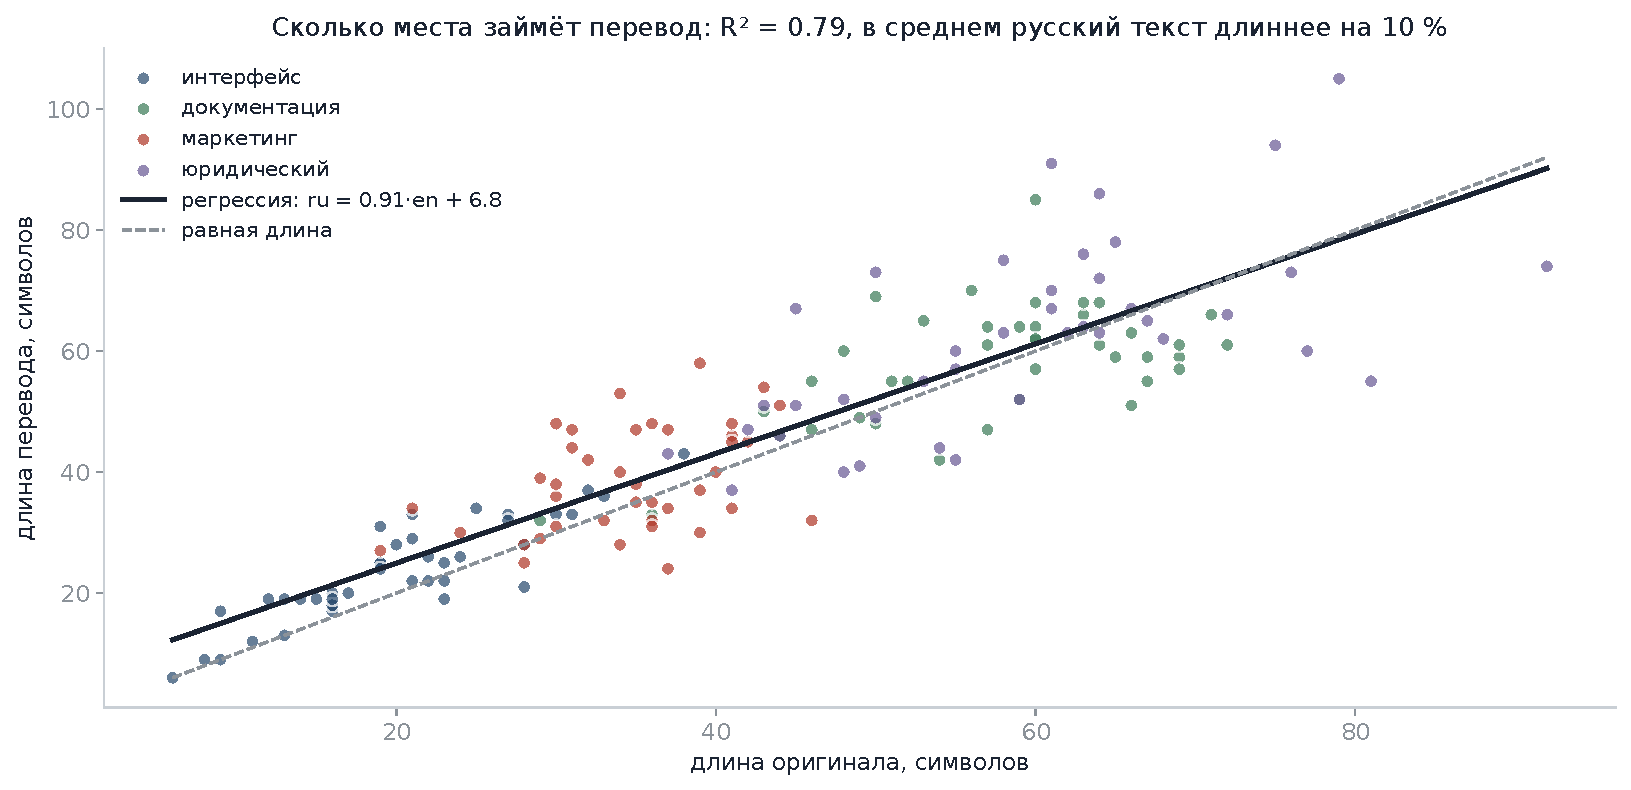
\includegraphics[width=0.76\textwidth]{fig/regression.pdf}
  \end{center}

  \vspace{-0.9em}
  {\small На нашем корпусе русский текст длиннее английского в среднем на
  \числ{10\,\%}, а не на пятнадцать. И разброс по типам контента больше
  самой поправки: интерфейс \числ{+20\,\%}, документация \числ{+2\,\%}.
  \textbf{Средний коэффициент, применённый ко всему проекту сразу,
  ошибается ровно там, где цена ошибки максимальна — на кнопках.}}
\end{frame}

% =====================================================================
\begin{frame}{Кластеризация}
  \framesubtitle{обучение без учителя}

  Разбиение множества объектов на группы, \textbf{заданные не человеком,
  а данными}. Разметки нет: машина сама решает, что на что похоже.

  \vspace{0.9em}
  \кейс{Как это выглядит в работе:} пришёл незнакомый корпус на 30 тысяч
  сегментов. Хочется разложить его на группы, чтобы оценить объём и
  назначить исполнителей до начала перевода.

  \vspace{0.9em}
  \врезка{\textbf{Предупреждение, которое лучше сделать заранее.}
  В Л.р.\,№\,2 кластеризация даст согласие с нашей разметкой около нуля.
  Это не сбой лабораторной и не ваша ошибка. Посмотрим, почему.}
\end{frame}

% =====================================================================
\begin{frame}{Что кластеризация находит на самом деле}
  \begin{center}
    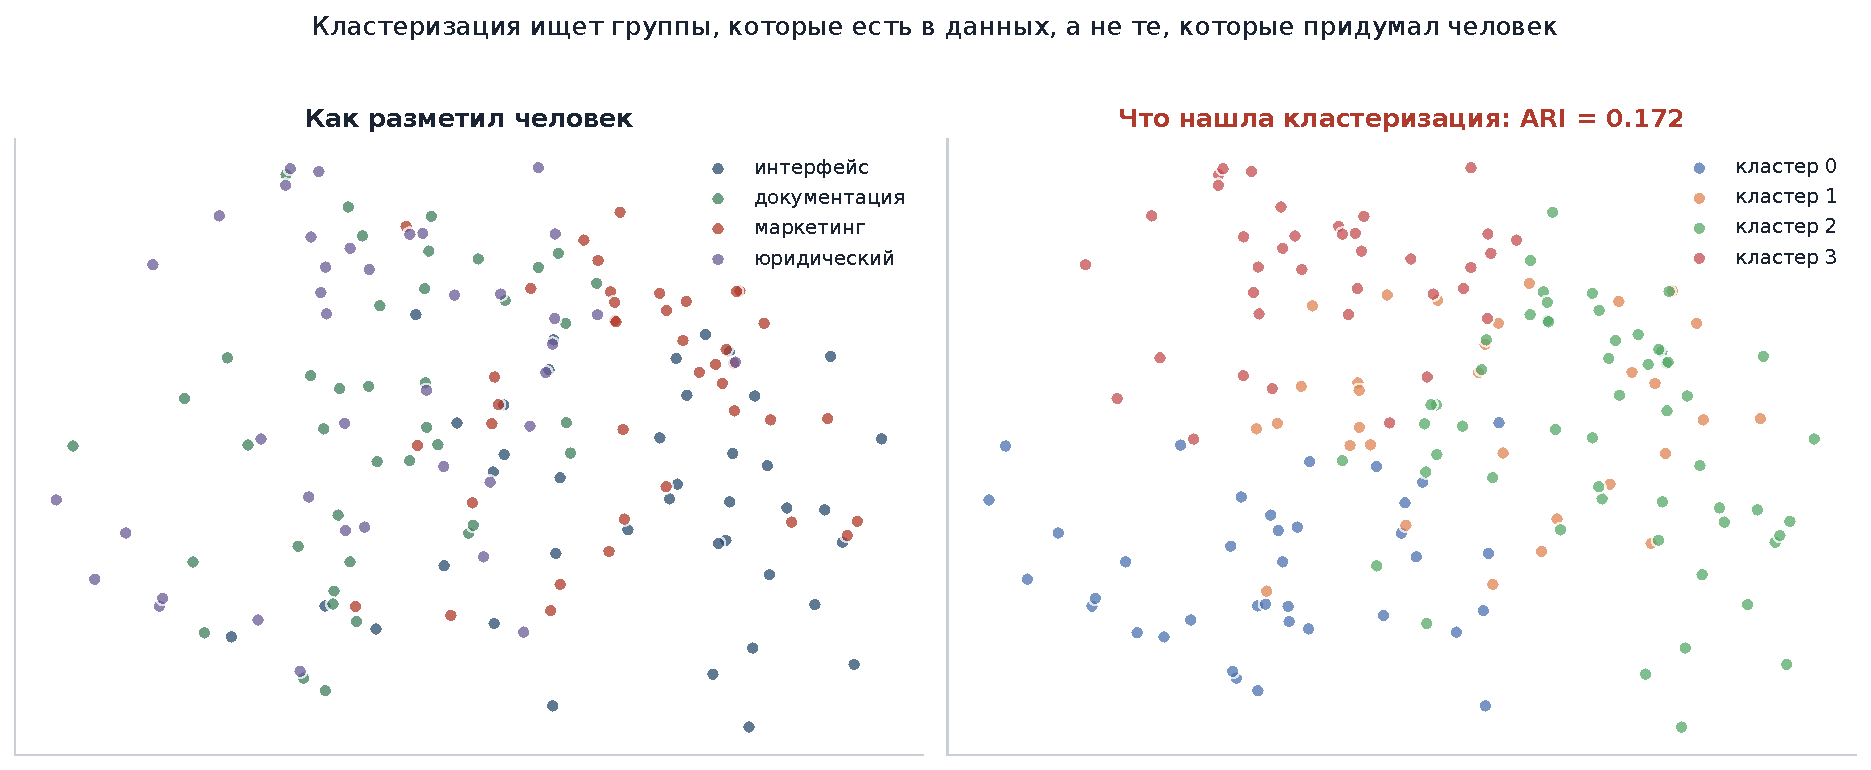
\includegraphics[width=0.90\textwidth]{fig/clusters.pdf}
  \end{center}

  \vspace{-0.4em}
  {\small ARI — мера согласия двух разбиений: \числ{1{,}0} — полное
  совпадение, \числ{0{,}0} — как если бы группы нарезали случайно.
  Получилось \числ{0{,}172}.}

  \playground{https://konkin-nikita.ru/gd_learn/tm/}{память переводов}%
  {ARI на трёх представлениях и разброс по восьми запускам.}
\end{frame}

% =====================================================================
\begin{frame}{Почему это правильный результат, а не поломка}
  Кластеризация честно нашла структуру, которая в данных есть. Просто это
  \textbf{не та структура}, которую придумал человек.

  \vspace{0.8em}
  {\small Машина сгруппировала сегменты по длине и доле служебной лексики —
  по тому, что сильнее всего различает тексты численно. Наши четыре типа
  контента различаются \emph{назначением}, а оно из формы видно лишь отчасти.}

  \vspace{1.0em}
  \врезка{\textbf{Правило, которое стоит унести с собой.} Кластеризация
  отвечает на вопрос «на какие группы эти данные распадаются сами».
  Она не отвечает на вопрос «разложи их по моим категориям» — для этого
  нужна разметка и классификация. Подбором числа кластеров заставить её
  воспроизвести разметку нельзя, и в Л.р.\,№\,2 вы это проверите.}
\end{frame}

% =====================================================================
\begin{frame}{Снижение размерности}
  \framesubtitle{обучение без учителя, оно же обобщение}

  Преобразование, которое \textbf{уменьшает число признаков}, стараясь
  сохранить то, что в данных существенно.

  \vspace{0.7em}
  {\small Тексты описываются тысячами признаков, и почти все они нули:
  конкретное буквосочетание встречается в считаных сегментах. Сжатие
  собирает из множества слабых признаков несколько сильных.}

  \vspace{0.9em}
  \врезка{Метод очень хорошо подходит для определения тематик текстов
  (\textit{topic modelling}) — и это прямая опора Л.р.\,№\,2, где
  \texttt{TruncatedSVD} и \texttt{PCA} применяются к нашему корпусу.
  Тот же приём лежит за «умными» подсказками в CAT-инструментах:
  подсказка ищется не по буквам, а по сжатому представлению смысла.}

  \playground{https://konkin-nikita.ru/gd_learn/tm/}{память переводов}%
  {один сегмент, четыре меры близости, и где они расходятся.}
\end{frame}

% =====================================================================
\begin{frame}{Сколько информации остаётся при сжатии}
  \begin{center}
    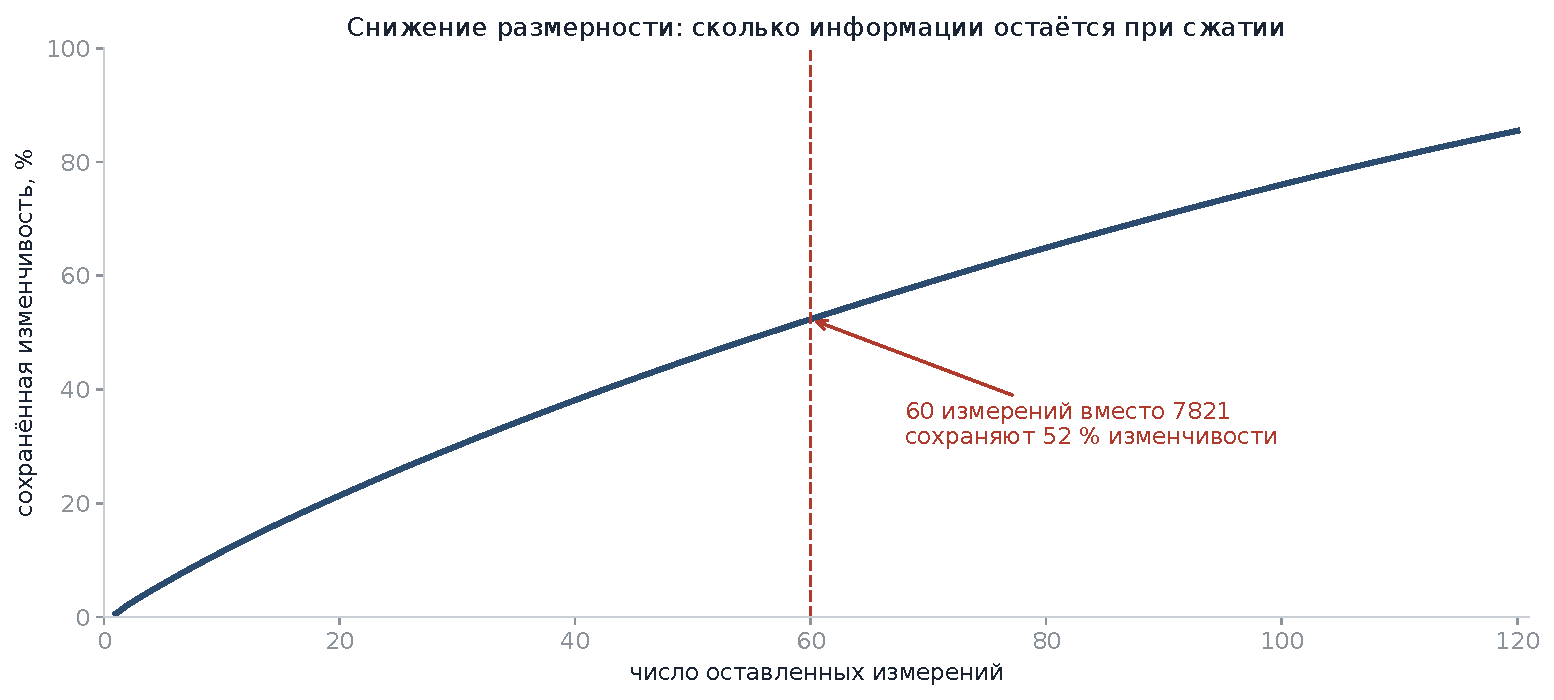
\includegraphics[width=0.74\textwidth]{fig/svd.pdf}
  \end{center}

  \vspace{-0.4em}
  {\small Сжатие в \числ{130} раз сохраняет половину изменчивости корпуса.
  Вторая половина — это то, чем сегменты отличаются друг от друга по
  мелочам, и для поиска похожего она чаще мешает, чем помогает.}
\end{frame}

% =====================================================================
\begin{frame}{Поиск правил (ассоциации)}
  \framesubtitle{обучение без учителя}

  Метод ищет, что в данных встречается \textbf{вместе}.

  \vspace{0.2em}
  \begin{center}
    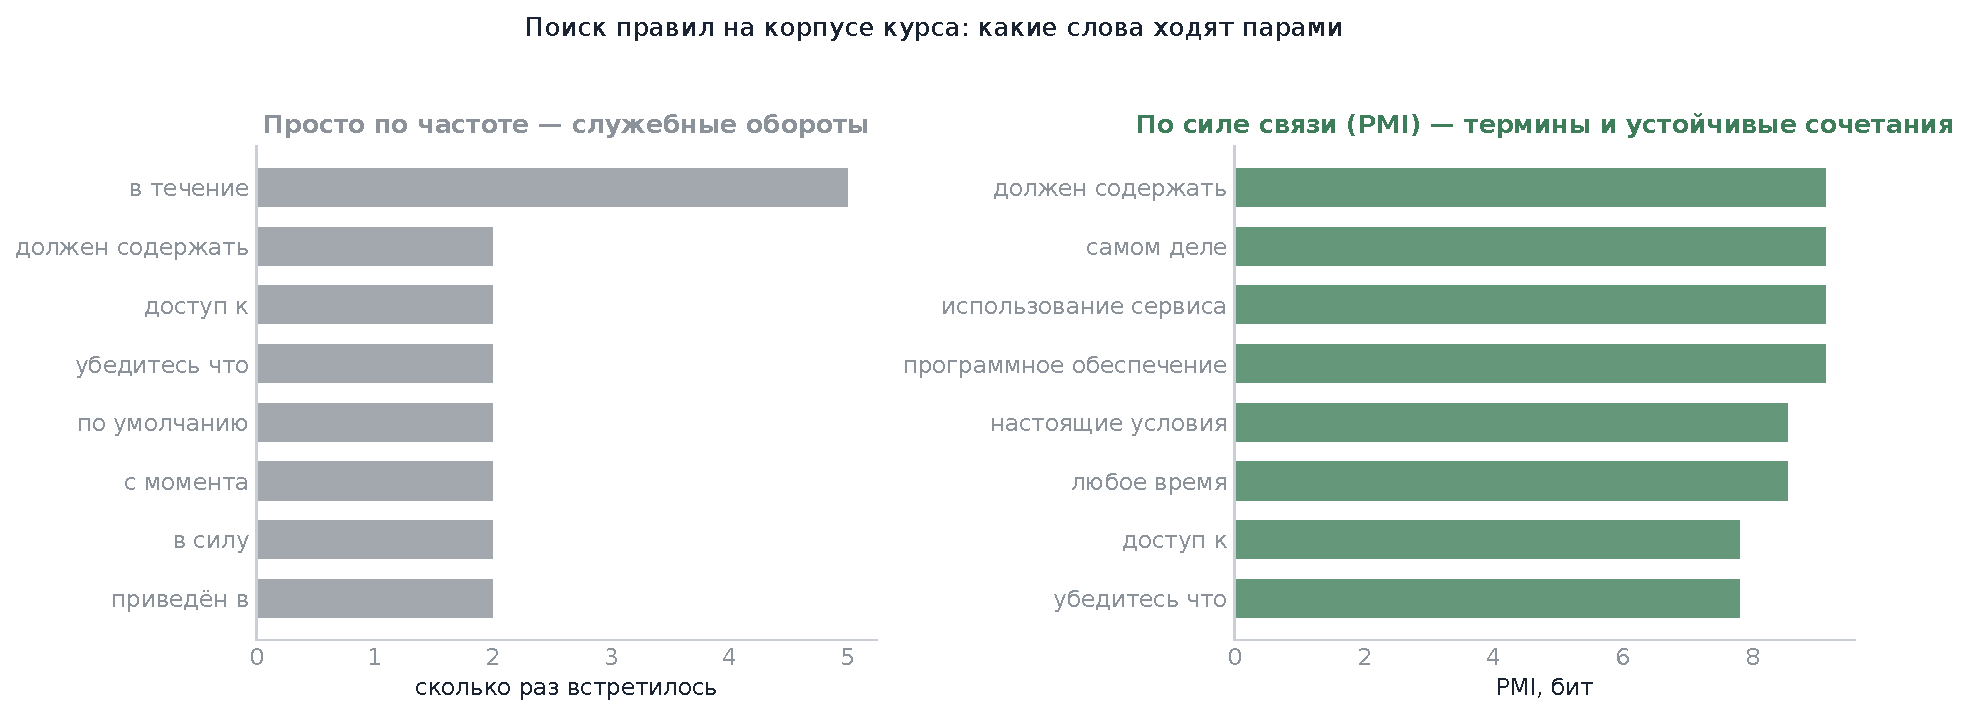
\includegraphics[width=0.78\textwidth]{fig/assoc.pdf}
  \end{center}

  \vspace{-0.6em}
  \врезка{\textbf{Слева — ловушка, справа — инструмент.} По частоте наверх
  всплывают служебные обороты. Мера силы связи (PMI) поднимает то, что
  действительно ходит парами: «программное обеспечение», «настоящие
  условия». Это заготовка глоссария, полученная за секунду, — её остаётся
  вычитать лингвисту.}
\end{frame}

% =====================================================================
\begin{frame}{Обучение с подкреплением}
  \framesubtitle{четвёртое направление — назовём и пойдём дальше}

  Модель не получает готовых ответов. Она \textbf{действует в среде} и
  получает отклик: награду или штраф. Так учат играть в го, водить
  автомобиль, управлять роботом.

  \vspace{1.0em}
  \врезка{\textbf{Почему в нашем курсе этого не будет.} Метод требует
  среды, в которой можно совершить действие и немедленно узнать, хорошим
  оно было или плохим. Перевод такой средой не является: оценку качества
  даёт человек, она приходит с задержкой в недели и стоит дороже самого
  перевода.\\[0.5em]
  Знать о направлении стоит, применять его в локализации — нет.}
\end{frame}

% =====================================================================
\begin{frame}{Ансамбли}
  Несколько несовершенных моделей, \textbf{исправляющих ошибки друг друга},
  работают лучше одной сильной.

  \vspace{0.8em}
  {\small Здесь работает бритва Оккама: задача должна решаться самым простым
  способом. Три простые модели, каждая из которых ошибается по-своему,
  обычно надёжнее одной сложной, которая ошибается вся сразу.}

  \vspace{0.8em}
  {\small Технические схемы — стекинг, бэггинг, бустинг — различаются тем,
  как именно модели соединяют. Собирать их руками вам не придётся; важна
  сама идея.}

  \vspace{1.0em}
  \врезка{\textbf{А вот идея вам пригодится буквально.} В Л.р.\,№\,3
  приёмка машинного перевода собрана ровно по этому принципу — из трёх
  разных средств, каждое из которых закрывает слепое пятно другого.}

  \playground{https://konkin-nikita.ru/gd_learn/mt/}{метрики перевода}%
  {сломать перевод и увидеть, что заметит каждое средство.}
\end{frame}

% =====================================================================
\begin{frame}{Ансамбль, собранный человеком}
  \begin{center}
    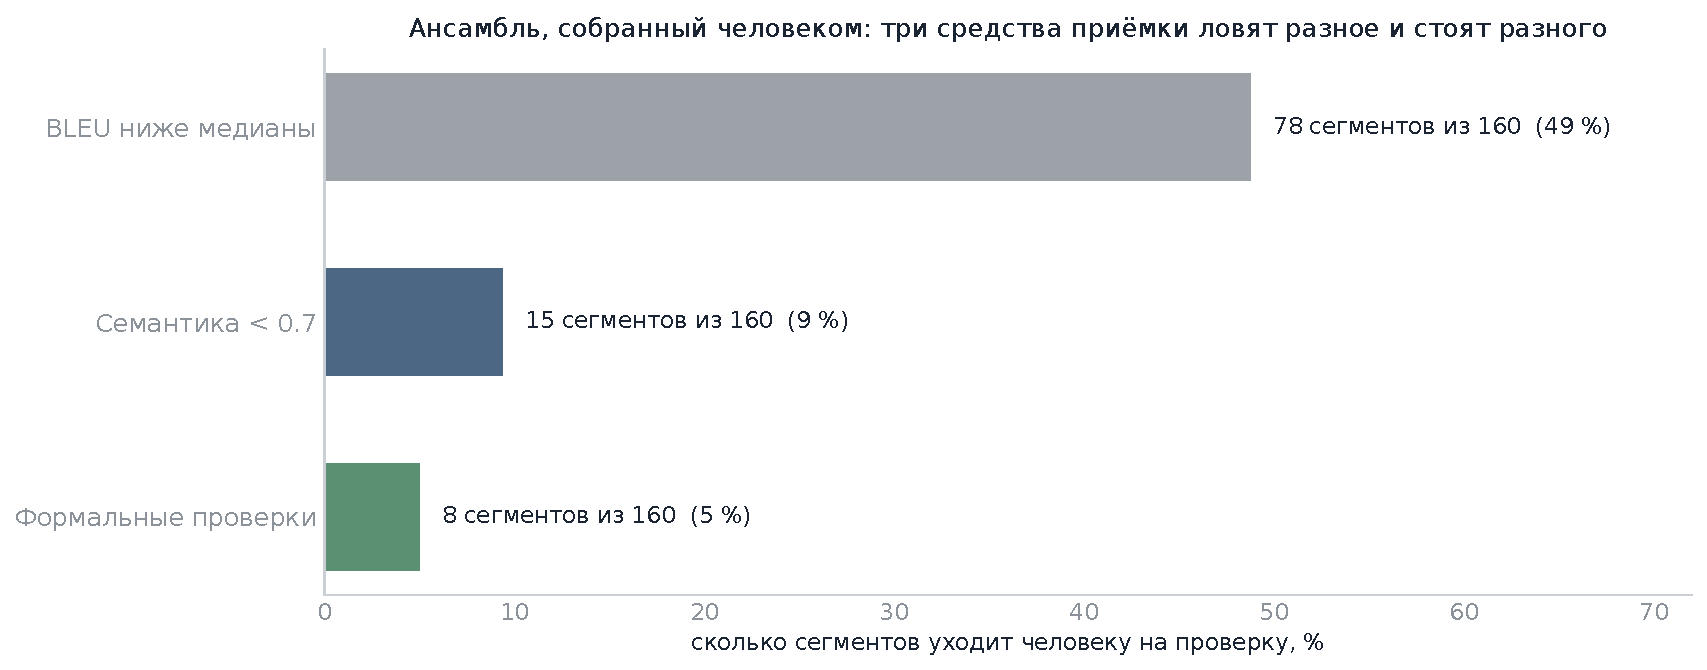
\includegraphics[width=0.86\textwidth]{fig/ensemble.pdf}
  \end{center}

  \vspace{-0.5em}
  {\small\textbf{Три средства ловят разное и стоят разного.} Метрика BLEU
  отправляет на проверку половину корпуса и при этом пропускает сегмент
  с разрушенным плейсхолдером \texttt{\{name\}} — его BLEU \emph{выше}
  медианы. Формальная проверка находит этот сегмент мгновенно и стоит
  восьми регулярных выражений.}
\end{frame}

% =====================================================================
\begin{frame}{Нейронные сети}
  \framesubtitle{глубокое обучение}

  Математическая модель, построенная по принципу сети нервных клеток.
  Состоит из \textbf{нейронов} и связей между ними — \textbf{синапсов}.

  \vspace{0.8em}
  {\small Нейрон — это функция: принимает несколько чисел на вход, умножает
  каждое на свой вес, складывает и пропускает сумму через функцию активации.
  Вся сеть — это много таких функций, соединённых слоями.}

  \vspace{1.0em}
  \врезка{Дальше — тот же пример, что был у дерева решений: определить
  тип сегмента. Так видно, чем нейрон отличается от правила, и почему
  «сеть научилась» — это всегда «подобрались числа».}
\end{frame}

% =====================================================================
\begin{frame}{Как устроен один нейрон}
  \begin{center}
    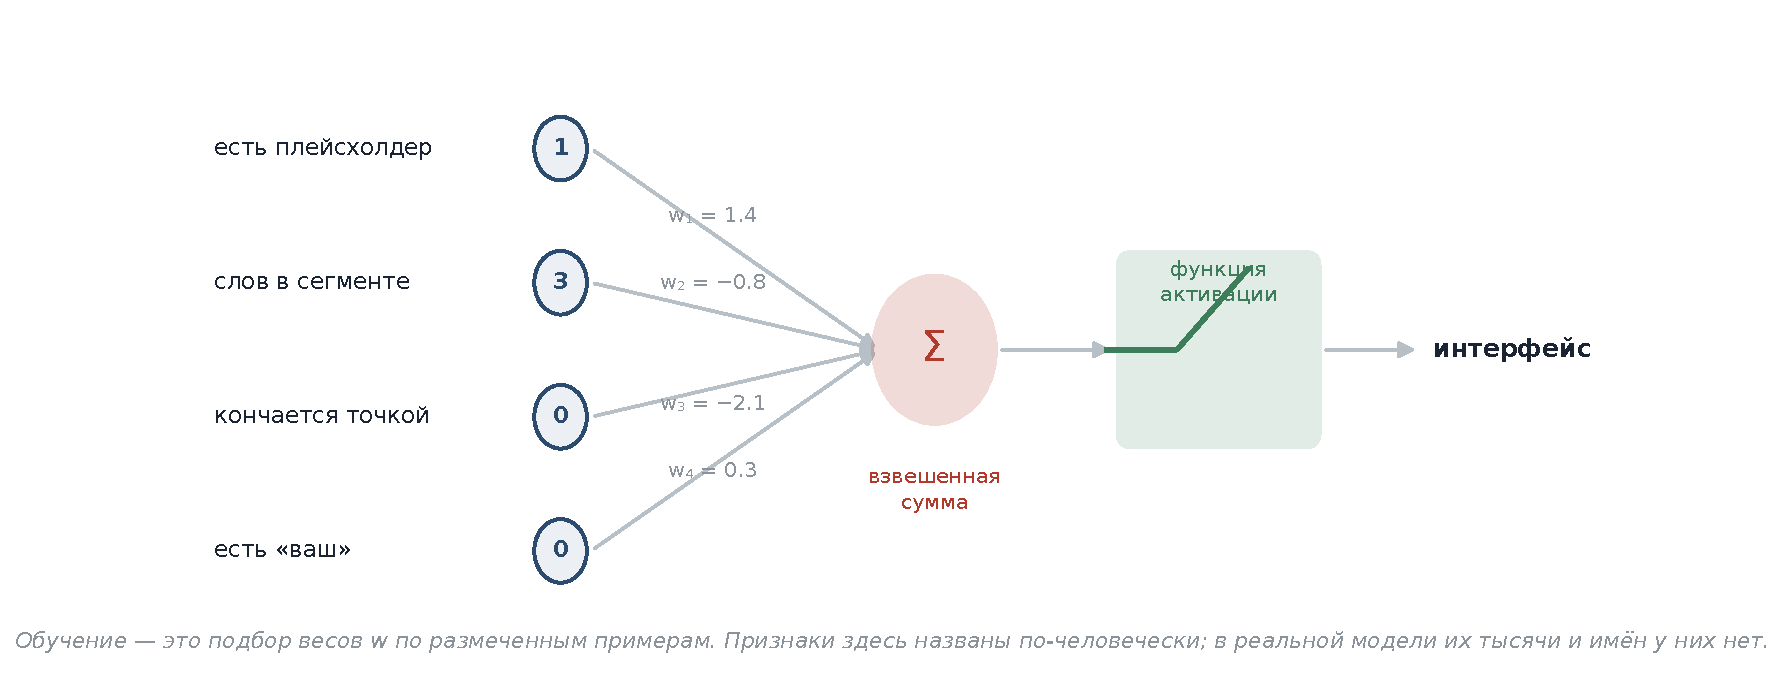
\includegraphics[width=0.93\textwidth]{fig/neuron.pdf}
  \end{center}

  \vspace{-0.8em}
  \врезка{\textbf{Здесь нет ничего, кроме арифметики.} Признаки умножаются
  на веса, произведения складываются, сумма проходит через функцию
  активации. Веса \числ{1{,}4}, \числ{-0{,}8}, \числ{-2{,}1}, \числ{0{,}3}
  никто не задавал — они подобраны по размеченным примерам. «Сеть
  научилась» всегда означает «подобрались числа».}
\end{frame}

% =====================================================================
\begin{frame}{Слои и обучение}
  \begin{columns}[T,onlytextwidth]
    \column{0.47\textwidth}
      {\color{navy}\bfseries Слои}\\[0.5em]
      {\small Нейроны выстраивают в слои. Внутри слоя связей нет, между
      соседними — есть.\par
      \vspace{0.6em}
      Смысл в том, что каждый следующий слой работает с признаками,
      которые предыдущий уже собрал, а не с исходным текстом.}
    \column{0.47\textwidth}
      {\color{navy}\bfseries Обучение}\\[0.5em]
      {\small Обучить сеть — значит \textbf{расставить веса} так, чтобы на
      обучающих примерах ответы совпадали с размеченными.\par
      \vspace{0.6em}
      Сеть отвечает, ошибку измеряют, веса чуть двигают туда, где ошибка
      меньше. Миллионы раз.}
  \end{columns}

  \vspace{0.4em}
  \врезка{\textbf{Отсюда следует вещь, важная для приёмки.} Сеть не знает
  правил и не может их назвать. Она не «понимает», что плейсхолдер
  \texttt{\{name\}} нельзя переводить, — она лишь редко видела обратное.
  Поэтому в Л.р.\,№\,3 плейсхолдеры проверяются регуляркой, а не моделью.}

  \playground{https://konkin-nikita.ru/gd_learn/}{градиентный спуск}%
  {«веса чуть двигают» — по шагам, с выбором шага и зерна.}
\end{frame}

% =====================================================================
\begin{frame}{Свёрточные сети}
  \framesubtitle{зачем мы их пропускаем}

  Архитектура, заточенная под изображения: сеть ищет в картинке простые
  линии, из них собирает фигуры, из фигур — объекты.

  \vspace{1.0em}
  \врезка{\textbf{В обработке текста их применяли, но они вытеснены
  трансформерами.} Для локализации архитектура не нужна ни разу, а на
  разбор уходит четверть часа. Мы эти пятнадцать минут потратим на
  устройство языковой модели — во второй презентации курса.}

  \vspace{1.0em}
  {\color{ash}\small Если встретите в вакансии «CNN» — это про
  компьютерное зрение, а не про вашу работу.}
\end{frame}

% =====================================================================
\begin{frame}{Рекуррентные сети}
  \framesubtitle{мост к Л.р.\,№\,4}

  Сети, в которых связи образуют цикл: выход шага подаётся на вход
  следующего. Так сеть получает \textbf{память о том, что было раньше} в
  последовательности, — а текст и есть последовательность.

  \vspace{0.9em}
  {\small Именно на этой архитектуре работал машинный перевод примерно с
  2014 по 2017 год, и именно её вы увидите в Л.р.\,№\,4: сеть посимвольно
  порождает текст, обучившись на корпусе.}

  \vspace{0.9em}
  \врезка{\textbf{Посмотрите на её вывод внимательно.} Он похож на язык,
  но рассыпается через несколько слов. Причина — у рекуррентной сети
  память короткая: к концу предложения начало уже размыто. Механизм
  внимания в трансформере придуман ровно против этого, и о нём —
  следующая презентация.}

  \playground{https://konkin-nikita.ru/gd_learn/lm/}{языковая модель}%
  {температура, top-k и top-p на символьной модели.}
\end{frame}

% =====================================================================
\begin{frame}{Итог: что где в курсе}
  \vspace{0.2em}
  {\footnotesize\setlength{\extrarowheight}{2pt}
  \begin{tabular}{@{}Л{0.27}Л{0.46}Л{0.19}@{}}
    \toprule
    \textbf{Задача} & \textbf{Наш случай} & \textbf{Где отрабатываем} \\
    \midrule
    Классификация &
      тип контента по тексту сегмента &
      {\color{brick}Л.р.\,№\,1} \\
    Регрессия &
      длина перевода по длине оригинала &
      разобрана здесь \\
    Кластеризация &
      разложить незнакомый корпус &
      {\color{brick}Л.р.\,№\,2} \\
    Снижение размерности &
      поиск по памяти переводов &
      {\color{brick}Л.р.\,№\,2} \\
    Поиск правил &
      заготовка глоссария из корпуса &
      разобран здесь \\
    Ансамбли &
      три средства приёмки перевода &
      {\color{brick}Л.р.\,№\,3} \\
    Нейронные сети &
      порождение текста, машинный перевод &
      {\color{brick}Л.р.\,№\,4} \\
    \bottomrule
  \end{tabular}}

  \vspace{0.4em}
  {\color{ash}\footnotesize Обучения с подкреплением в таблице нет намеренно.}
\end{frame}

% =====================================================================
\begin{frame}{Где всё это можно потрогать руками}
  \framesubtitle{\href{https://konkin-nikita.ru/gd_learn/}{konkin-nikita.ru/gd\_learn/}}

  {\small Пять страниц на корпусе этого курса: те же числа, что в
  лабораторных, прямо в браузере.}

  \vspace{0.4em}
  {\footnotesize\setlength{\extrarowheight}{2pt}
  \begin{tabular}{@{}Л{0.22}Л{0.44}Л{0.14}@{}}
    \toprule
    \textbf{Тема лекции} & \textbf{Что крутится} & \textbf{Страница} \\
    \midrule
    Обучение сети &
      шаг, зерно, форма функции потерь &
      \href{https://konkin-nikita.ru/gd_learn/}{\texttt{/}} \\
    Классификация &
      слова против символьных n-грамм, стемминг &
      \href{https://konkin-nikita.ru/gd_learn/vec/}{\texttt{/vec/}} \\
    Кластеризация, снижение размерности &
      четыре меры близости на одном запросе; ARI и разброс &
      \href{https://konkin-nikita.ru/gd_learn/tm/}{\texttt{/tm/}} \\
    Ансамбли &
      сломать перевод и увидеть, что заметит каждое средство &
      \href{https://konkin-nikita.ru/gd_learn/mt/}{\texttt{/mt/}} \\
    Рекуррентные сети &
      температура, top-k и top-p на символьной модели &
      \href{https://konkin-nikita.ru/gd_learn/lm/}{\texttt{/lm/}} \\
    \bottomrule
  \end{tabular}}
\end{frame}

% =====================================================================
\begin{frame}{Что унести с этой лекции}
  \begin{enumerate}
    \item\small \textbf{Модель без точки отсчёта — число без единиц измерения.}
      Прежде чем радоваться точности, посмотрите, сколько даёт решение,
      вообще не читающее текст. У нас это \числ{0{,}25}.
      \vspace{0.5em}
    \item\small \textbf{Признаки решают больше, чем алгоритм.} Смена модели —
      \числ{+0{,}01}, смена способа превратить текст в числа — \числ{+0{,}21}.
      \vspace{0.5em}
    \item\small \textbf{Понятность и точность — разные вещи, и за них платят
      по-разному.} Дерево \числ{0{,}631} и объяснимо, символьные n-граммы
      \числ{0{,}744} и нет.
      \vspace{0.5em}
    \item\small \textbf{Отрицательный результат — тоже результат.}
      Кластеризация не воспроизводит разметку, и это свойство метода,
      а не сбой.
      \vspace{0.5em}
    \item\small \textbf{Средний коэффициент врёт там, где дороже всего.}
      Перевод длиннее на \числ{10\,\%} в среднем и на \числ{20\,\%} в
      интерфейсе — а место кончается именно на кнопках.
  \end{enumerate}
\end{frame}

\end{document}
